%\documentclass[final, onecolumn, 3p]{elsarticle}
\documentclass[..]{../IEEEphot}
\usepackage{array,multirow}

%******************************************
%*************** My packages **************
%******************************************
\usepackage{amsmath}
\usepackage{amssymb}
\usepackage{booktabs}
\usepackage[utf8]{inputenc}
\usepackage{longtable}
\usepackage{times}
\usepackage[italian]{babel}
\usepackage{textcomp}
\usepackage[svgnames]{xcolor}
\usepackage{scalerel}
\usepackage{keystroke}
%******************************************
%******************************************
%******************************************


%******************************************
%*************** My commands **************
%******************************************

%Circled characters
\makeatletter
\usepackage{tikz}
\usetikzlibrary{calc}
\newcommand*\circled[1]{\tikz[baseline=(char.base)]{
    \node[shape=circle, draw, inner sep=1pt, 
        minimum height={\f@size*1.6},] (char) {\vphantom{WAH1g}#1};}}
\makeatother
%******************************************
%******************************************
%******************************************

\newcommand{\param}[1]{\colorbox{LightSlateGray}{\color{Navy}\texttt{\textbf{#1}}}}

\newcolumntype{z}[1]{>{\centering\arraybackslash}m{#1}}% a centered m-type column
\renewcommand*\multirowsetup{\centering}% default is \raggedright

\def\msquare{\mathord{\scalerel*{\Box}{gX}}}



\begin{document}

\title{AutoCAD$^{\text{\textregistered}}$ cheat sheet}

\author{Francesco~Bianconi}

\affil{Dipartimento di Ingegneria\\ Università degli Studi di Perugia \\ Via Goffredo Duranti, 93 -- 06125 Perugia (Italy)\\ \texttt{bianco@ieee.org} \\} 

\maketitle
% * <john.hammersley@gmail.com> 2015-02-09T12:07:31.197Z:
%
%  Click the title above to edit the author information and abstract
%
\thispagestyle{empty}

\vspace{-1.0cm}
\noindent Aggiornato alla versione 2022 di AutoCAD (alcuni comandi potrebbero non funzionare con versioni precedenti). Ultima revisione: \today.

\tableofcontents

\clearpage

\section{Sistemi di riferimento ed inserimento delle coordinate}
\begin{longtable}{m{.3\linewidth}>{\centering\arraybackslash}p{.3\linewidth}>{\centering\arraybackslash}p{.3\linewidth}}
\toprule
\multirow{2}{*}{Sistema di riferimento} & \multicolumn{2}{c}{Tipo di coordinate} \\
\cmidrule{2-3}
 & Cartesiane & Polari \\
\midrule
Globale (WCS) & \multicolumn{1}{c}{*$x$,$y$} & \multicolumn{1}{c}{*$\rho<\theta$} \\
Utente (UCS) & \multicolumn{1}{c}{$x$,$y$} & \multicolumn{1}{c}{$\rho<\theta$} \\
Locale & \multicolumn{1}{c}{@$x$,$y$} & \multicolumn{1}{c}{@$\rho<\theta$} \\
\bottomrule
\end{longtable}

\section{Comandi per la creazione di entità grafiche}

\begin{center}
\begin{longtable}{m{.1\linewidth}m{.2\linewidth}m{.3\linewidth}m{.3\linewidth}}
\toprule
    \multicolumn{2}{c}{\bfseries Comando} &
    \multicolumn{1}{c}{\bfseries Funzione} &
    \multicolumn{1}{c}{\bfseries Principali parametri} \\
\midrule
\texttt{\_arc} & 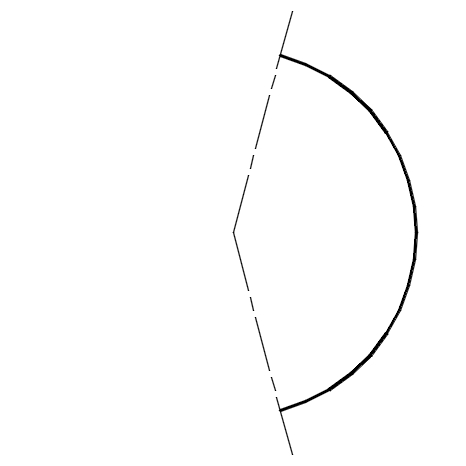
\includegraphics[width = 0.8\linewidth, keepaspectratio]{../images/jpg/_arc.jpg}
& Genera un arco di circonferenza. & 
\param{C}: permette di specificare il centro dell'arco (al posto del punto iniziale).
\\			
\midrule
\texttt{\_circle} & 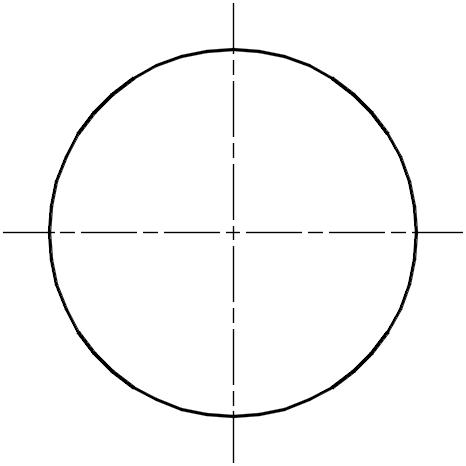
\includegraphics[width = 0.8\linewidth, keepaspectratio]{../images/jpg/_circle.jpg} 
& Genera una circonferenza completa. & 
\param{D}: permette di specificare il diametro della circonferenza (al posto del raggio).

\param{3P}: genera una circonferenza dati tre punti.

\param{2P}: genera una circonferenza dati due punti (diametralmente opposti).

\param{T}: genera una circonferenza dati tre segmenti ad essa tangenti.
\\	

\midrule
\texttt{\_ellipse} & 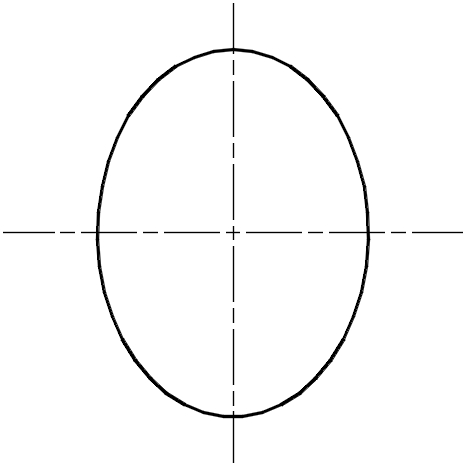
\includegraphics[width = 0.8\linewidth, keepaspectratio]{../images/jpg/_ellipse.jpg}
& Genera un ellisse o un arco di ellisse. & 
\param{A}: genera un arco di ellisse (invece di un'ellisse completa).

\param{C}: genera un'ellisse partendo dal centro.
\\
\midrule
\texttt{\_hatch} & 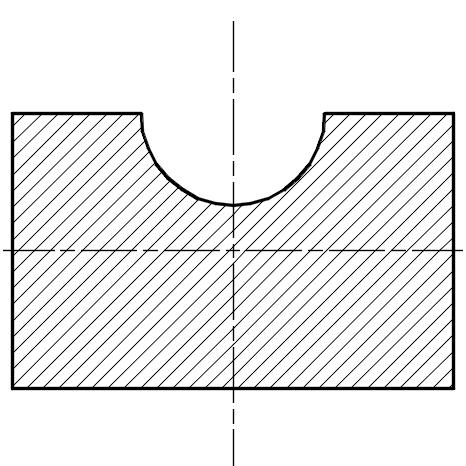
\includegraphics[width = 0.8\linewidth, keepaspectratio]{../images/jpg/_hatch.jpg} & Genera la campitura (tratteggio) di una regione chiusa & 
\\
\midrule
\texttt{\_line} & 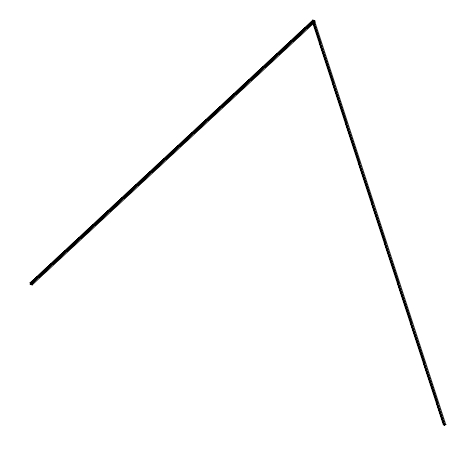
\includegraphics[width = 0.8\linewidth, keepaspectratio]{../images/jpg/_line.jpg} & Genera una linea o una spezzata (polilinea). & 
\param{C}: chiude la spezzata (attivo se sono definiti più di due punti). \\
\midrule
\texttt{\_point} & 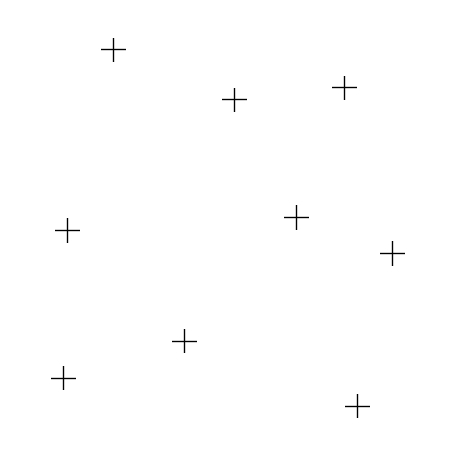
\includegraphics[width = 0.8\linewidth, keepaspectratio]{../images/jpg/_point.jpg} & Genera un punto. &  \\	
\midrule
\texttt{\_polygon} & 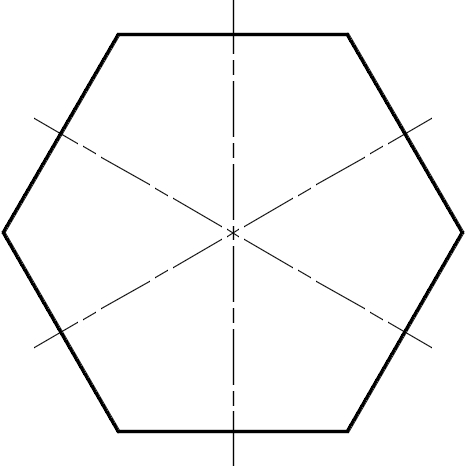
\includegraphics[width = 0.8\linewidth, keepaspectratio]{../images/jpg/_polygon.jpg} & Genera un poligono regolare di $n$ lati inscritto o circoscritto ad una circonferenza. & 
\param{C}: genera un poligono circoscritto ad una circonferenza.

\param{I}: genera un poligono inscritto ad una circonferenza.  \\
\midrule
\texttt{\_rectang} & 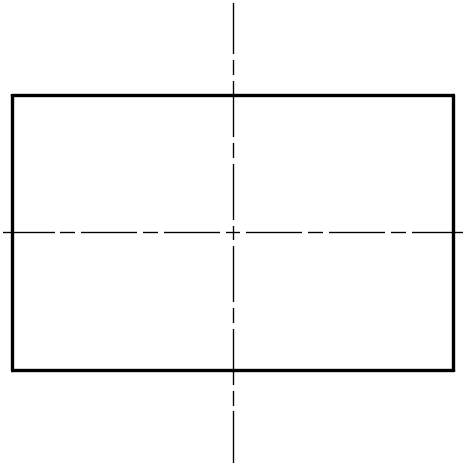
\includegraphics[width = 0.8\linewidth, keepaspectratio]{../images/jpg/_rectang.jpg} & Genera un rettangolo. & 
\param{C}: definisce le dimensioni dello smusso ai vertici.

\param{R}: definisce le dimensioni del raccordo ai vertici.

\param{Q}: definisce le dimensioni del rettangolo (larghezza ed altezza).

\\
\bottomrule
\end{longtable}
\end{center}

\clearpage

\section{Comandi per la modifica di entità grafiche}

\begin{center}
\begin{longtable}{m{.2\linewidth}m{.2\linewidth}m{.25\linewidth}m{.25\linewidth}}
\toprule
    \multicolumn{2}{c}{\bfseries Comando} &
    \multicolumn{1}{c}{\bfseries Funzione} &
    \multicolumn{1}{c}{\bfseries Principali parametri} \\
\midrule
\texttt{\_arrayclassic} & 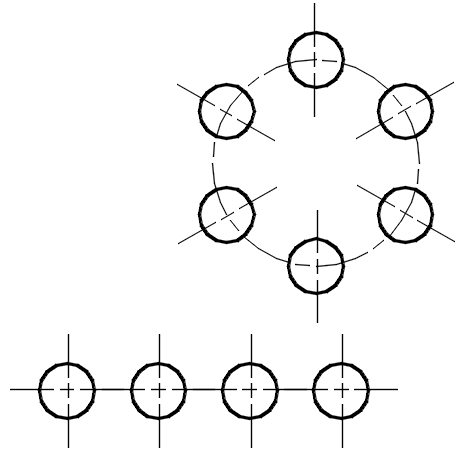
\includegraphics[width = 0.8\linewidth, keepaspectratio]{../images/jpg/_arrayclassic.jpg} & Esegue una ripetizione lineare o circolare (polare) di uno o più oggetti. & 
\\
\midrule
\texttt{\_chamfer} & 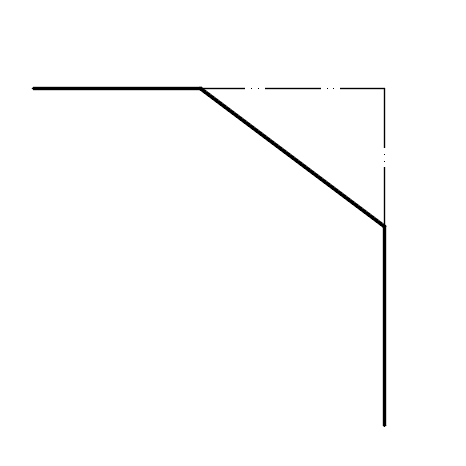
\includegraphics[width = 0.8\linewidth, keepaspectratio]{../images/jpg/_chamfer.jpg}  
& Crea uno smusso tra due linee. È necessario che le due linee (o i loro prolungamenti) si intersechino. & 
\param{D}: definisce il valore delle distanze di smusso. L'ordine con cui vengono assegnate le distanze corrisponde all'ordine cui vengono selezionate le linee.
\\
\midrule
\texttt{\_copy} & 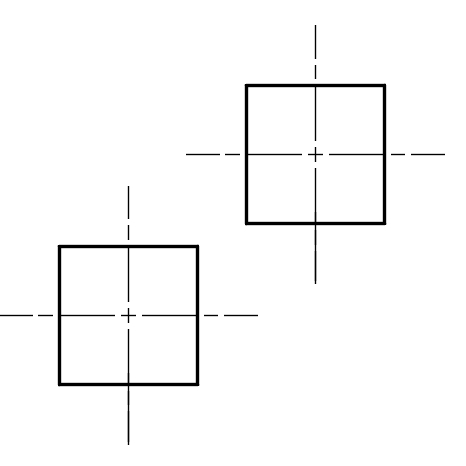
\includegraphics[width = 0.8\linewidth, keepaspectratio]{../images/jpg/_copy.jpg} & Copia un oggetto od un gruppo di oggetti. & 
\param{S}: specifica il vettore spostamento
\\	
\midrule
\texttt{\_erase} & & Elimina un oggetto od un gruppo di oggetti. Equivale alla pressione del tasto \keystroke{Canc}. & 
\\	
\midrule
\texttt{\_explode} & & Divide un oggetto o un gruppo di oggetti in parti separate (opposto di \texttt{\_join}). & 
\\	
\midrule
\texttt{\_extend} & 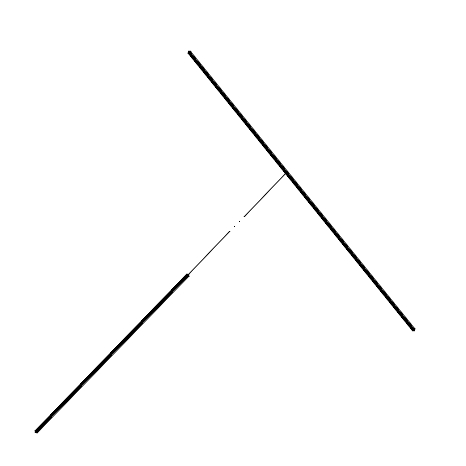
\includegraphics[width = 0.8\linewidth, keepaspectratio]{../images/jpg/_extend.jpg} & Prolunga uno o più oggetti fini ad incontrare un altro oggetto (limite dell'estensione). Occorre selezionare prima il limite dell'estensione e poi l'oggetto da estendere.  & 
\\	
\midrule
\texttt{\_fillet} & 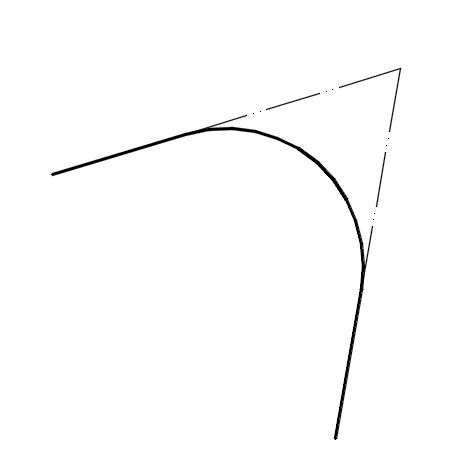
\includegraphics[width = 0.8\linewidth, keepaspectratio]{../images/jpg/_fillet.jpg} & Crea un raccordo tra due linee. È necessario che le due linee (o i loro prolungamenti) si intersechino. & 
\param{RA}: definisce il valore del raggio di raccordo.
\\
\midrule
\texttt{\_intersect} & 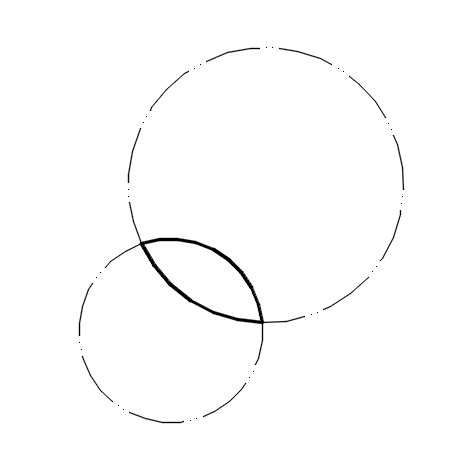
\includegraphics[width = 0.8\linewidth, keepaspectratio]{../images/jpg/_intersect.jpg} & Intersezione booleana (AND) tra due figure chiuse. È necessario che le due figure siano previamente convertite in regioni attraverso il comando \texttt{\_region}. & 
\\
\midrule
\texttt{\_join} & & Unisce linee, polilinee, spline ed archi contigui (opposto di \texttt{\_explode}). & 
\\
\midrule
\texttt{\_mirror} & 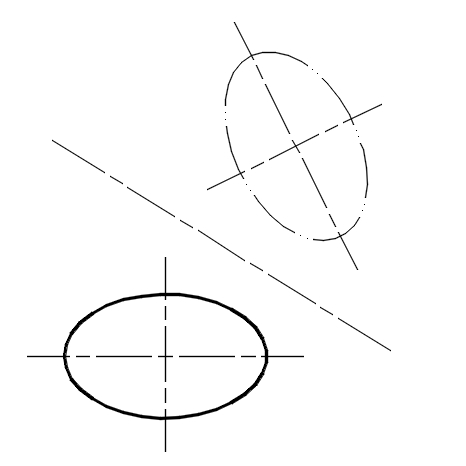
\includegraphics[width = 0.8\linewidth, keepaspectratio]{../images/jpg/_mirror.jpg} & Riflette un oggetto o un gruppo di oggetti rispetto ad un asse. & 
\param{N}: gli oggetti sorgente non vengono cancellati (esegue una copia).

\param{S}: gli oggetti sorgente vengono cancellati.
\\		
\midrule
\texttt{\_move} & 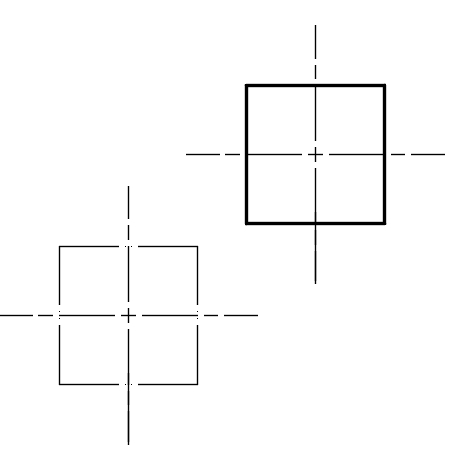
\includegraphics[width = 0.8\linewidth, keepaspectratio]{../images/jpg/_move.jpg} & Sposta un oggetto o un gruppo di oggetti. & 
\param{S}: specifica il vettore spostamento.
\\			
\midrule
\texttt{\_offset} & 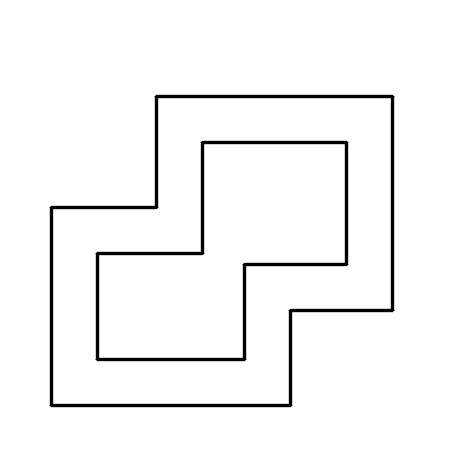
\includegraphics[width = 0.8\linewidth, keepaspectratio]{../images/jpg/_offset.jpg} & Crea una copia di un oggetto mantenendo uno spessore assegnato rispetto all'oggetto originale.  & 
\\			
\midrule
\texttt{\_rotate} & 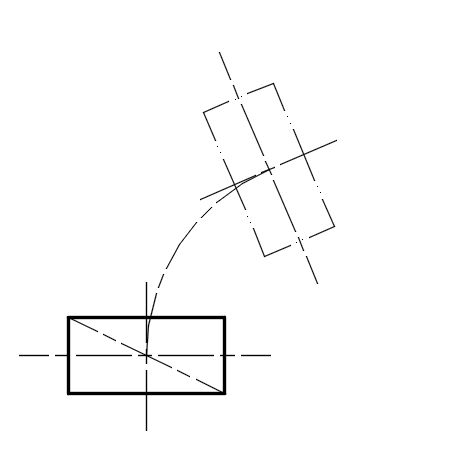
\includegraphics[width = 0.8\linewidth, keepaspectratio]{../images/jpg/_rotate.jpg} & Ruota un oggetto od un gruppo di oggetti. & 
\param{C}: crea una copia (gli oggetti sorgente non vengono cancellati).
\\	
\midrule
\texttt{\_scale} & 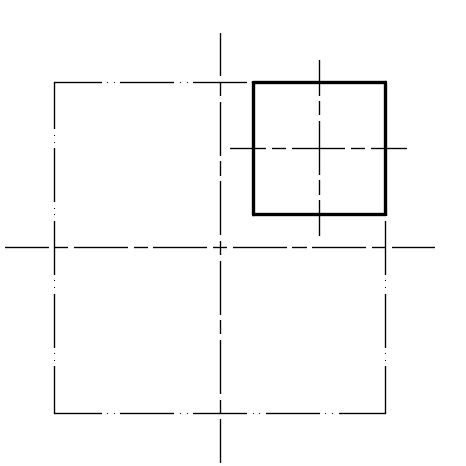
\includegraphics[width = 0.8\linewidth, keepaspectratio]{../images/jpg/_scale.jpg} & Applica una trasformazione di scala ad uno o più oggetti. & 
\param{C}: crea una copia (gli oggetti sorgente non vengono cancellati).
\\	
\midrule
\texttt{\_subtract} & 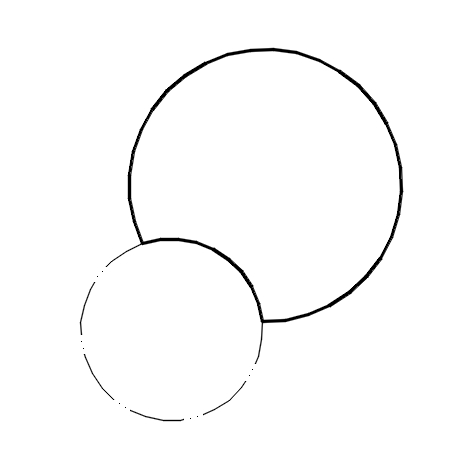
\includegraphics[width = 0.8\linewidth, keepaspectratio]{../images/jpg/_subtract.jpg} & Differenza booleana tra due figure chiuse. È necessario che le due figure siano previamente convertite in regioni attraverso il comando \texttt{\_region}. & 
\\
\midrule
\texttt{\_trim} & 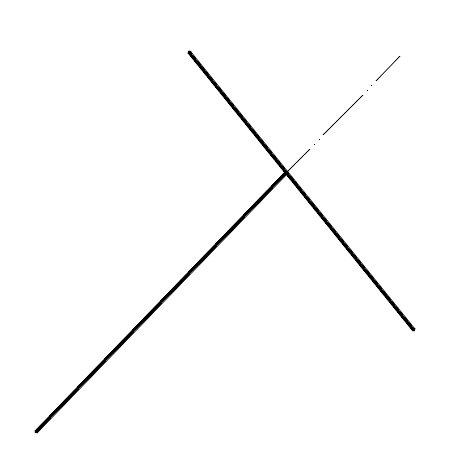
\includegraphics[width = 0.8\linewidth, keepaspectratio]{../images/jpg/_trim.jpg} & Ritaglia uno o più oggetti utilizzando altri oggetti come utensili di taglio. Si selezionano prima gli oggetti utensile e poi quelli da tagliare.  & 
\\	
\midrule
\texttt{\_union} & 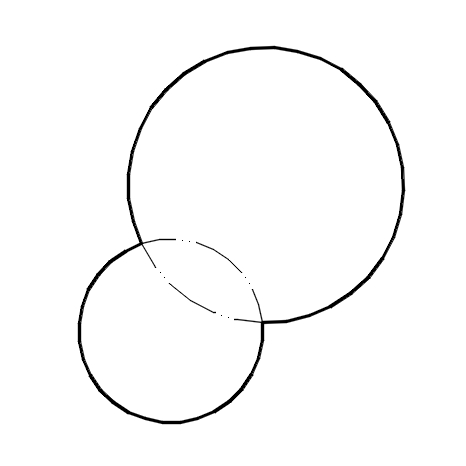
\includegraphics[width = 0.8\linewidth, keepaspectratio]{../images/jpg/_union.jpg} & Unione booleana (OR) tra due figure chiuse. È necessario che le due figure siano previamente convertite in regioni attraverso il comando \texttt{\_region}. & 
\\
\bottomrule
\end{longtable}
\end{center}

\clearpage

\section{Comandi per l'inserimento delle quote e la modifica degli stili}

\begin{center}
\begin{longtable}{m{.2\linewidth}m{.2\linewidth}m{.25\linewidth}m{.25\linewidth}}
\toprule
    \multicolumn{2}{c}{\bfseries Comando} &
    \multicolumn{1}{c}{\bfseries Funzione} &
    \multicolumn{1}{c}{\bfseries Principali parametri} \\
\midrule
\texttt{\_dimlinear} & 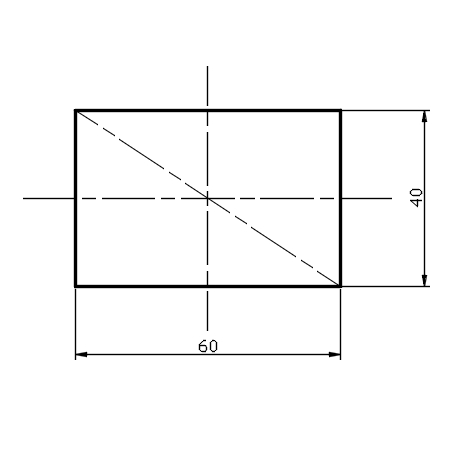
\includegraphics[width = 0.8\linewidth, keepaspectratio]{../images/jpg/_dimlinear.jpg} & Inserisce una quota parallela ad uno degli assi del sistema UCS. & 
\\
\midrule
\texttt{\_dimaligned} & 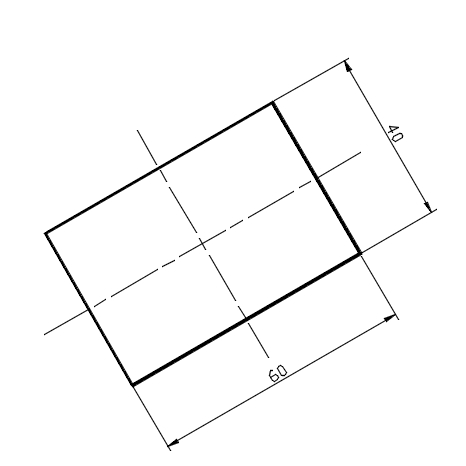
\includegraphics[width = 0.8\linewidth, keepaspectratio]{../images/jpg/_dimaligned.jpg} & Inserisce una quota parallela ad un segmento sghembo rispetto agli assi del sistema UCS. & 
\\
\midrule
\texttt{\_dimdiameter} & 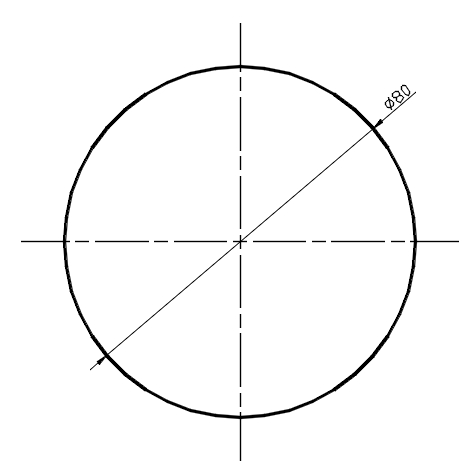
\includegraphics[width = 0.8\linewidth, keepaspectratio]{../images/jpg/_dimdiameter.jpg} & Inserisce una quota diametro. & 
\\
\midrule
\texttt{\_dimradius} & 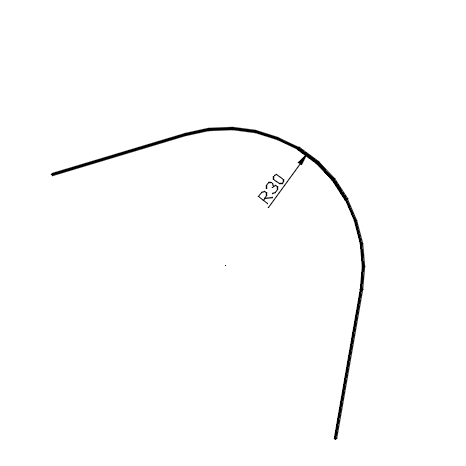
\includegraphics[width = 0.8\linewidth, keepaspectratio]{../images/jpg/_dimradius.jpg} & Inserisce una quota raggio. & 
\\
\midrule
\texttt{\_dimstyle} & & Visualizza la finestra che permette la gestione degli stili di quota. & 
\\
\bottomrule
\end{longtable}
\end{center}

\clearpage

\section{Comandi per l'inserimento del testo e delle annotazioni}

\begin{center}
\begin{longtable}{m{.2\linewidth}m{.2\linewidth}m{.25\linewidth}m{.25\linewidth}}
\toprule
    \multicolumn{2}{c}{\bfseries Comando} &
    \multicolumn{1}{c}{\bfseries Funzione} &
    \multicolumn{1}{c}{\bfseries Principali parametri} \\
\midrule
\texttt{\_mtext} & 
\includegraphics[width = 0.8\linewidth, keepaspectratio]{../images/jpg/_mtext.jpg} & Inserisce del testo multilinea. & 
\param{A}: imposta l'altezza del carattere.

\param{G}: modifica l'ancoraggio del testo e/o adatta la larghezza del carattere (vedi \texttt{\_text}).

\param{SP}: imposta lo spazio tra i caratteri.
\\
\midrule
\texttt{\_qleader} & 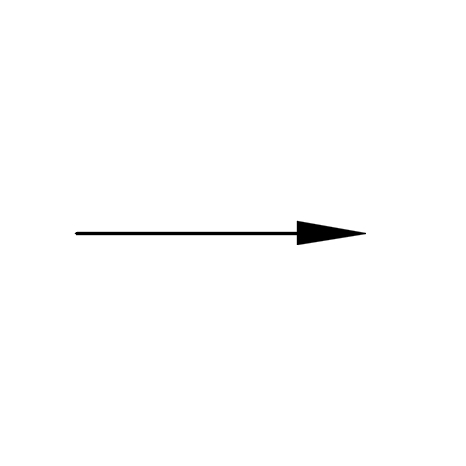
\includegraphics[width = 0.8\linewidth, keepaspectratio]{../images/jpg/_qleader.jpg} & Genera una freccia. \\
\midrule
\texttt{\_text} & 
\includegraphics[width = 0.8\linewidth, keepaspectratio]{../images/jpg/_text.jpg} & Inserisce del testo a riga singola. & 
\param{G}: modifica l'ancoraggio del testo e/o adatta la larghezza del carattere. Alcune possibili opzioni:
\begin{itemize}
\item \param{AS} (ancoraggio in alto a sinistra)
\item \param{AC} (ancoraggio in alto al centro)
\item \param{AD} (ancoraggio in alto a destra)
\item \param{MS} (ancoraggio in mezzo a sinistra)
\item \param{MC} (ancoraggio in mezzo al centro)
\item \param{MD} (ancoraggio in mezzo a destra)
\item \param{BS} (ancoraggio in basso a sinistra)
\item \param{BC} (ancoraggio in basso al centro)
\item \param{BD} (ancoraggio in basso a destra)
\item \param{T} (adatta la larghezza del carattere alla lunghezza complessiva della linea di testo).
\end{itemize}
\\
\midrule
\texttt{\_tolerance} & 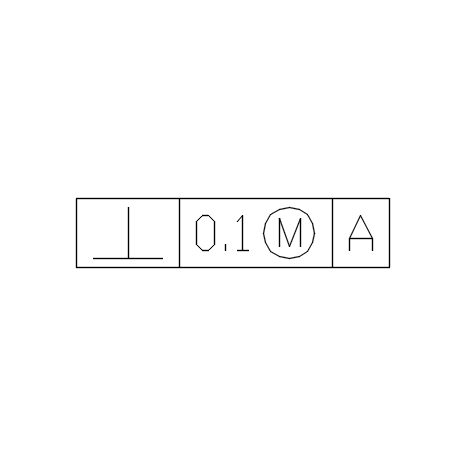
\includegraphics[width = 0.8\linewidth, keepaspectratio]{../images/jpg/_tolerance.jpg} & Genera simboli per tolleranze geometriche. \\
\midrule
\texttt{\_centerline} & 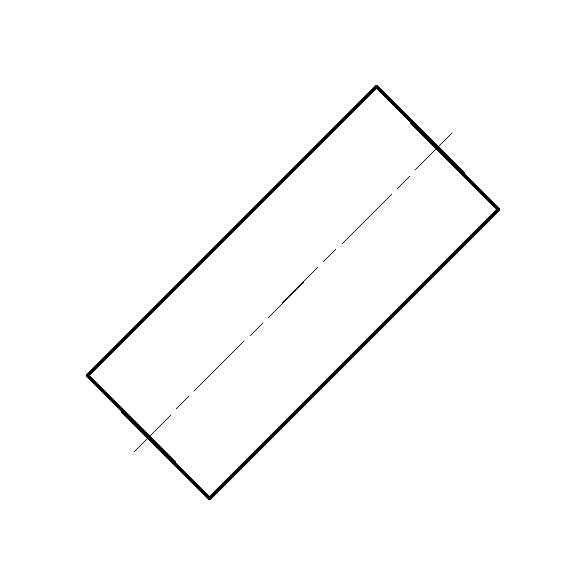
\includegraphics[width = 0.8\linewidth, keepaspectratio]{../images/jpg/_centerline.jpg} & Disegna l'asse mediano tra due rette parallele. & 
\\
\midrule
\texttt{\_centermark} & 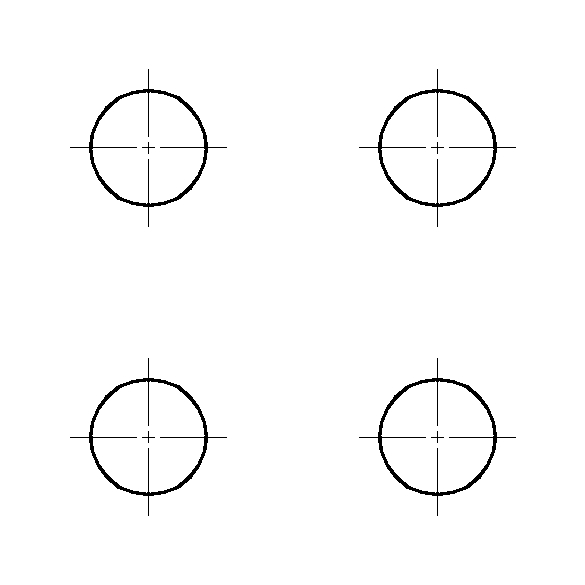
\includegraphics[width = 0.8\linewidth, keepaspectratio]{../images/jpg/_centermark.jpg} & Disegna gli assi di una circonferenza. & 
\\
\bottomrule
\end{longtable}
\end{center}

\subsection{Inserimento di caratteri speciali}

\vspace{\baselineskip}

\begin{center}
\begin{tabular}{lccc}
\toprule
\textbf{Denominazione} & \textbf{Simbolo} & \textbf{Sequenza AutoCAD} & \textbf{Sequenza Unicode}\\
\midrule
Diametro & \o & \%\%c & \textbackslash U+00B0 \\
\midrule
Esigenza d'inviluppo & \circled{E} & -- & \textbackslash U+24BA \\
\midrule
Gradi & $^{\circ}$ & \%\%d & \textbackslash U+2205 \\
\midrule
Più o meno & $^{\pm}$ & \%\%p & \textbackslash U+00B1  \\
\midrule
Quadrato & $\msquare$ & -- & \textbackslash U+25A1 \\
\bottomrule
\end{tabular}
\end{center}

\noindent
 

\subsection{Inserimento di caratteri speciali attraverso font \texttt{gdt}}

\vspace{\baselineskip}

\begin{center}
\begin{tabular}{lcc}
\toprule
\textbf{Denominazione} & \textbf{Simbolo} & \textbf{Sequenza AutoCAD} \\
\midrule
Diametro & \o & n \\
\midrule
Quadrato & $\msquare$ & o \\
\midrule
\raisebox{0pt}{Lamatura} & 
\includegraphics[width = 10pt, keepaspectratio]{../images/jpg/hole-counterbore.jpg} & \raisebox{0pt}{v} \\
\midrule
\raisebox{0pt}{Svasatura} & 
\includegraphics[width = 10pt, keepaspectratio]{../images/jpg/hole-countersink.jpg} & \raisebox{0pt}{w} \\
\midrule
\raisebox{5pt}{Profondità} & 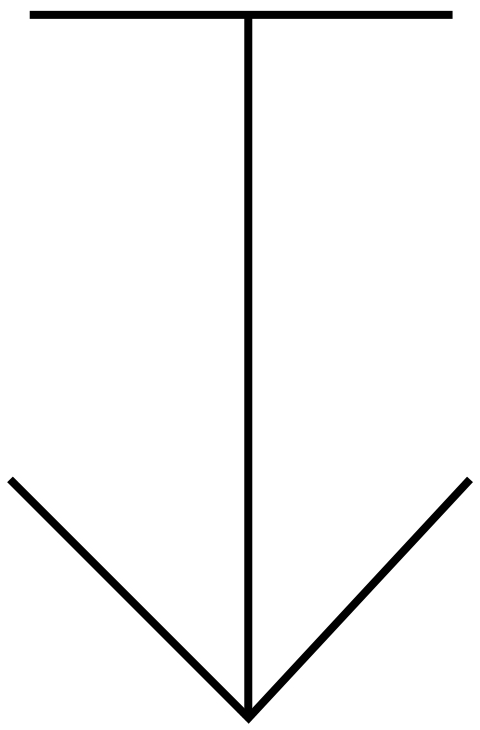
\includegraphics[width = 10pt, keepaspectratio]{../images/jpg/hole-depth.jpg} & \raisebox{5pt}{x} \\
\midrule
Conicità & 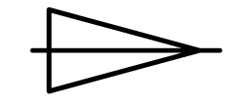
\includegraphics[height=\fontcharht\font`\B, keepaspectratio]{../images/jpg/GDandT_Conical_Taper_Symbol.jpg} & y \\
\midrule
Massimo materiale & \circled{M} & m \\
\midrule
Minimo materiale & \circled{L} & l \\
\bottomrule
\end{tabular}
\end{center}

\clearpage

\section{Comandi per il controllo del sistema, dell'interfaccia utente e delle proprietà degli oggetti}
\begin{center}
\begin{longtable}{m{.2\linewidth}m{.33\linewidth}m{.33\linewidth}}
\toprule
    \multicolumn{1}{c}{\bfseries Comando} &
    \multicolumn{1}{c}{\bfseries Funzione} &
    \multicolumn{1}{c}{\bfseries Principali parametri} \\
\midrule
\texttt{\_dynmode} & Attiva/disattiva la modalità input dinamico. & 
\param{1}: attiva la modalità input dinamico.

\param{0}: disattiva la modalità input dinamico.
\\
\midrule
\texttt{\_layer} & Apre la finestra che permette la creazione, rimozione e modifica delle proprietà dei layer. & 
\\
\midrule
\texttt{\_matchprop} & Assegna ad uno o più oggetti le proprietà dell'oggetto sorgente (equivalente a copia formato di Microsoft Word). & 
\\
\midrule
\texttt{\_navbardisplay} & Attiva/disattiva la visualizzazione della barra di navigazione. & 
\param{1}: attiva la visualizzazione della barra di navigazione.

\param{0}: disattiva la visualizzazione della barra di navigazione.
\\
\midrule
\texttt{\_orthomode} & Attiva/disattiva la modalità disegno ortogonale. & 
\param{1}: attiva la modalità disegno ortogonale.

\param{0}: disattiva la modalità disegno ortogonale.
\\
\midrule
\texttt{\_osnap} & Apre la finestra che permette la gestione degli snap ad oggetto. & 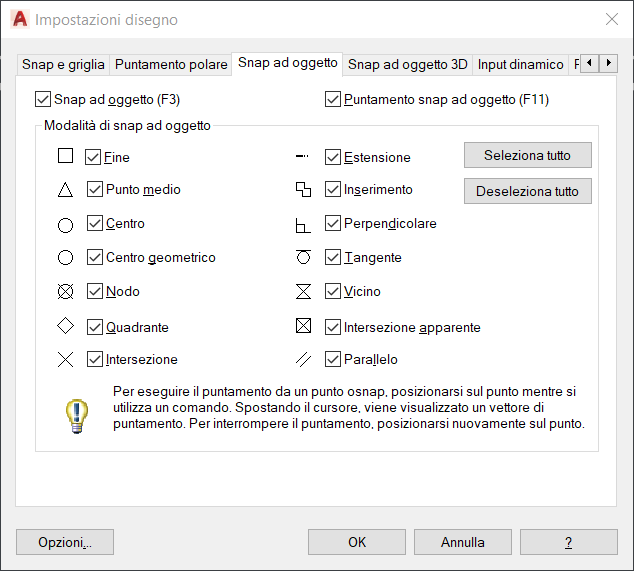
\includegraphics[width = 0.8\linewidth, keepaspectratio]{../images/png/_osnap.png}
\\
\midrule
\texttt{\_polarmode} & Attiva/disattiva la modalità disegno ad angoli predefiniti. & 
\param{1}: attiva la modalità disegno ad angoli predefiniti.

\param{0}: disattiva la modalità disegno ad angoli predefiniti.
\\
\midrule
\texttt{\_ptype} & Attiva la finestra per la modifica dello stile punti  & 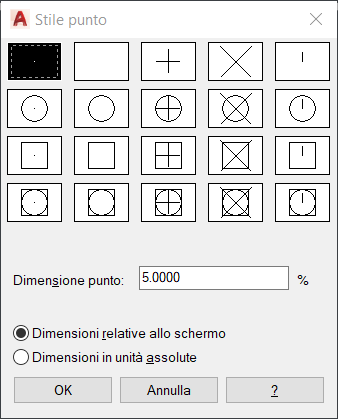
\includegraphics[width = 0.8\linewidth, keepaspectratio]{../images/png/_ptype.png} 
\\
\midrule
\texttt{\_qselect} & Attiva la finestra di selezione rapida di oggetti & 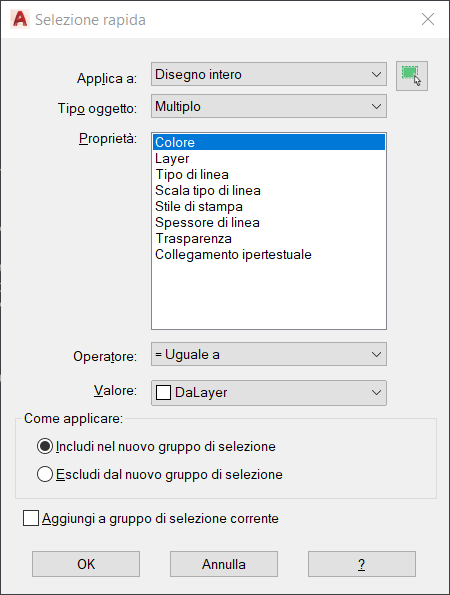
\includegraphics[width = 0.8\linewidth, keepaspectratio]{../images/png/_qselect.png} 
\\
\midrule
\texttt{\_regen} & Rigenera l'intero disegno. Ricalcola le posizioni e la visibilità di tutti gli oggetti contenuti nella finestra corrente. & 
\\
\midrule
\texttt{\_redraw} & Rigenera la visualizzazione nella finestra corrente. & 
\\
\midrule
\texttt{\_ucs} & Sposta il sistema di riferimento utente (UCS). & 
\\
\midrule
\texttt{\_ucsicon} & Attiva/disattiva la visualizzazione del sistema di riferimento utente (UCS). & 
\param{ON}: visualizza l'icona UCS.

\param{OF}: disattiva la visualizzazione dell'icona UCS.

\param{OR}: visualizza l'icona in corrispondenza dell'origine (0,0,0) dell'UCS corrente.
\\
\midrule
\texttt{\_units} & Permette di impostare le unità di misura del disegno e la precisione (numero di cifre decimali) delle dimensioni lineari ed angolari.
\\
\bottomrule
\end{longtable}
\end{center}

\clearpage

\section{Principali scorciatoie da tastiera}

\begin{center}
\begin{longtable}{m{.2\textwidth}m{.7\textwidth}m{.1\textwidth}}
\toprule
    \multicolumn{1}{c}{\bfseries Tasto} &
    \multicolumn{1}{c}{\bfseries Funzione/i}\\
\midrule
\keystroke{Canc} & Cancella gli oggetti selezionati. \\
\midrule
\keystroke{Ctrl}+\keystroke{B} & Attiva/disattiva lo snap a griglia. \\
\midrule
\keystroke{Ctrl}+\keystroke{O} & Apre un disegno esistente. \\
\midrule
\keystroke{Ctrl}+\keystroke{Q} & Chiude il programma. \\
\midrule
\keystroke{Ctrl}+\keystroke{Z} & Elimina l'ultima operazione eseguita. \\
\midrule
\keystroke{Ctrl}+\keystroke{Y} & Ripristina l'ultima operazione eseguita (annulla l'annullamento). \\
\midrule
\keystroke{Ctrl}+\keystroke{9} & Visualizza/nasconde la riga dei comandi. \\
\midrule
\keystroke{Esc} & 
Esce da un comando. 

Deseleziona tutti gli oggetti selezionati.
\\
\midrule
\keystroke{Invio} & 
Termina un comando, l'inserimento di un parametro o la selezione di oggetti all'interno di un comando. 

Ripete l'ultimo comando eseguito.
\\
\midrule
\keystroke{F3} & 
Attiva/disattiva gli snap ad oggetto.\\
\midrule
\keystroke{F8} & 
Attiva/disattiva la modalità di disegno `ortogonale'.\\
\midrule
\keystroke{F10} & 
Attiva/disattiva la modalità di disegno `puntamento polare'.\\
\midrule
\keystroke{F11} & 
Attiva/disattiva il puntamento ad oggetto (linee di riferimento).\\
\midrule
\keystroke{F12} & 
Attiva/disattiva la modalità di `input dinamico'.\\
\midrule
\keystroke{$\Uparrow$}, \keystroke{Shift} & 
Premuto assieme al tasto sinistro del mouse permette di rimuovere (deselezionare) uno o più oggetti da un insieme di selezione. \\
\bottomrule
\end{longtable}
\end{center}

\end{document}